\documentclass{fkpset}

% \newgeometry{bmargin=1in, tmargin=1.25in, lmargin=.75in, rmargin=.75in}
% \fancyhfoffset[R]{.05cm}

\name{Forest Kobayashi}
\class{Math 147}
\duedate{03/27/2019}
\assignment{HW 6 Solutions}

\chead{HW 6 Sample Solutions}
\rhead{Math 147 -- Spring, 2019}

\lfoot{Wednesday, March 27th 2019}

\problems{5.29, 5.32, 6.6, 6.11, 6.18}

\usepackage{hyperref}

\usetikzlibrary{hobby}

\newcommand{\tstd}{\ensuremath \ms T_{\rm std}}
\newcommand{\tprod}{\ensuremath \ms T_{\rm prod}}

\begin{document}
\pagestyle{plain}
\pagestyle{fancy}
  % \vspace{-2.9cm}
  \pointstable{}

  \vspace{1cm}

% --------------------------- Problem 1 ---------------------------- %
  \begin{problem}[5.29 (The Normality Lemma)]
    Let $A$ and $B$ be subsets of a topological space $X$ and let
    $\set{U_i}_{i \in \NN}$ and $\set{V_i}_{i \in \NN}$ be two
    collections of open sets such that
    \begin{enumerate}[label=(\arabic*)]
      \item $A \subset \bigcup_{i \in \NN} U_i$
      \item $B \subset \bigcup_{i \in \NN} V_i$
      \item For each $i \in \NN$, $\ol{U_i} \cap B = \varnothing$ and
        $\ol{V_i} \cap A = \varnothing$.
    \end{enumerate}
    Then there exist open sets $U$ and $V$ such that $A \subset U$, $B
    \subset V$, and $U \cap V = \varnothing$.
  \end{problem}
  \begin{leftbar}
    Before a solution, I'll give some intuition on how we might arrive
    at the candidate $U,V$ that work.

    Let's think about what we're given. We have $\set{U_i}_{i \in
      \NN}$, and $\set{V_i}_{i \in \NN}$ as defined above, and we want
    to use them to construct $U,V$ satisfying the given constraints.
    It seems like it'd be straightforward to satisfy $A \subset U$, $B
    \subset V$ --- they look like they'll probably fall directly out
    of the conditions. $U \cap V = \varnothing$ is harder, since we're
    given no direct information about $U_i \cap V_j$. Hence, we'll
    pick the following as our general approach:
    \begin{enumerate}[label=(\arabic*)]
      \item Think about what
        \[
          \tilde U = \bigcup_{i \in \NN} U_i \qquad\qquad \tilde V =
          \bigcup_{i \in \NN} V_i
        \]
        look like. In particular, we'll focus on the conditions that
        break/make $\tilde U$ and $\tilde V$ \emph{not} work as
        choices of $U,V$. Then,
      \item We'll see if we can find a clever way to remove the parts
        of $U_i$ and $V_i$ that cause problems. If all goes right,
        we'll find sequences $\set{U'_i}_{i\in\NN}$,
        $\set{V'_i}_{i\in\NN}$ whose terms can be unioned to get
        $U,V$.
    \end{enumerate}
    Depict our two sets $A,B$ as
    follows:
    \begin{center}
      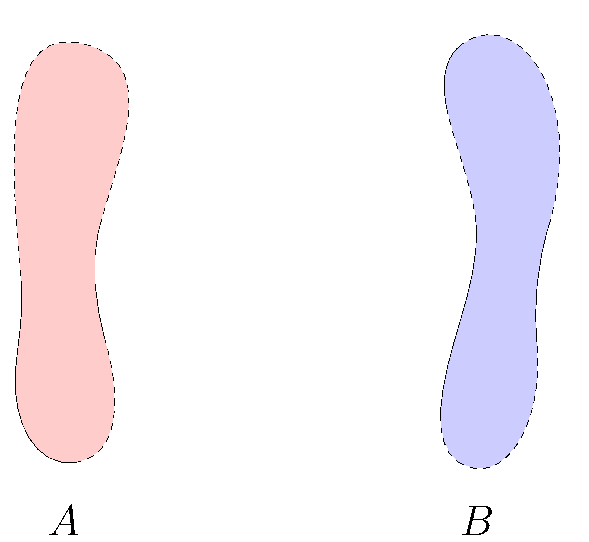
\includegraphics[keepaspectratio,width=6cm]{figures/5-29-AB}
    \end{center}
    To make the TikZ easier, I'll draw our covers with boxes --- but
    note, in general they could be blobby. Anyways, we now draw
    $U_1, V_1$:
    \begin{center}
      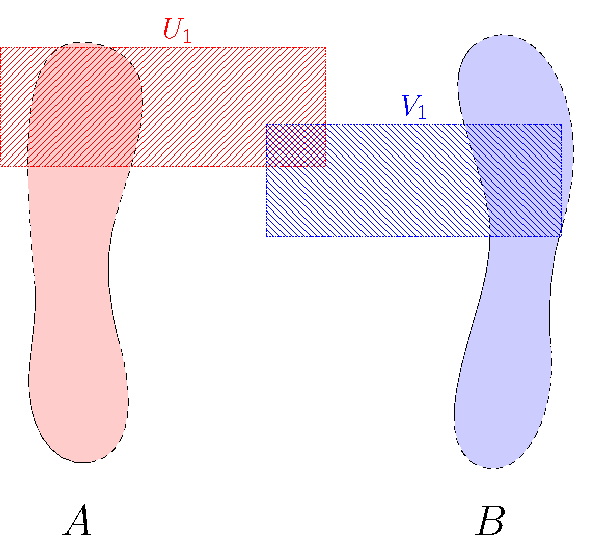
\includegraphics[keepaspectratio,width=6cm]{figures/5-29-n=1}
    \end{center}
    We need to be sure that in our construction of $U$, we don't
    include any of the $V_i$. We want to use the $U_i$, but as we can
    see, they might intersect the $V_i$. The fix? Remove the parts
    that cause problems. We define
    \begin{align*}
      U_1'
      &= U_1 - \ol{V_1}
      &
      V_1'
      &= V_1 - \ol{U_1}
    \end{align*}
    which yields
    \begin{center}
      \includegraphics[keepaspectratio, width=6cm]{figures/5-29-n=1-primes}
    \end{center}
    Now, we consider $n=2$:
    \begin{center}
      \includegraphics[keepaspectratio, width=6cm]{figures/5-29-n=2}
    \end{center}
    We already know how to rectify $U_1, V_1$:
    \begin{center}
      \includegraphics[keepaspectratio, width=6cm]{figures/5-29-n=2-prime1}
    \end{center}
    but we still have a problem now. Our addition of $U_2, V_2$ is
    complicating the situation! Namely, we have $U_2 \cap V'_1 \neq
    \varnothing$, $U_2 \cap V_2 \neq \varnothing$.\footnote{Note we
      could also have the analogous for $V_2 \cap U'_1$ if $V_2$ were
      a bit larger.} We \emph{don't} want to go back and edit our
    definitions for $U'_1, V'_1$ --- if we were to take this approach,
    we'd need to proceed similarly for $n=2$, $n=3$, etc.\ until
    eventually $U'_1 = U_1 - \bigcup_{i\in\NN} \ol{V_i}$, which could
    cause some problems.

    Instead, we'll modify $U_2$ and $V_2$, leaving $U'_1$ and $V'_1$
    untouched. Hence, we let
    \[
      U'_2 = U_2 - (\ol{V_1} \cup \ol{V_2}) \qquad\qquad
      V'_2 = V_2 - (\ol{U_1} \cup \ol{U_2})
    \]
    which gives us
    \begin{center}
      \includegraphics[keepaspectratio, width=6cm]{figures/5-29-n=2-prime2}
    \end{center}
    From which we can see $(U'_1 \cup U'_2) \cap (V'_1 \cup V'_2) \neq
    \varnothing.$ Thus, we conjecture that in the general case,
    \[
      U'_n = U_n - \bigcup_{i=1}^n \ol{V_i} \qquad\qquad V'_n = V_n -
      \bigcup_{i=1}^n \ol{U_i}
    \]
    will work.
  \end{leftbar}
  \begin{solution}

  \end{solution}
  \clearpage

% --------------------------- Problem 2 ---------------------------- %

  \begin{problem}[5.32]
    Suppose a space $X$ is regular and has a countable basis. Then $X$
    is normal.
  \end{problem}
  \begin{solution}
    Let $A,B$ be disjoint closed sets.
  \end{solution}
  \clearpage

% --------------------------- Problem 3 ---------------------------- %
  \begin{problem}[6.6]
    The space $2^\RR$ is separable.
  \end{problem}
  \begin{solution}
    We first find a candidate countable dense subset. As a candidate,
    we consider the set of all finite unions of intervals with
    rational endpoints:
    \begin{leftbar}
      Let
      \[
        S = \set{\bigcup_{i=1}^n (p_i, q_i) \MID n \in \NN,\
          \text{and}\ p_i, q_i \in \QQ \text{ for each $i$}}.
      \]
      First, note that the set comprehension above is at most
      countable (the set of all finite subsets of a countable set is
      countable). Hence, $S$ is at most countable as well.

      Now, note that $S$ has a countably infinite subset:
      \[
        S' = \set{(0,q) \MID q \in \QQ} \subset S.
      \]
      Thus $S$ is at least countable as well, and so $\abs{S} =
      \abs{\NN}$. \cmark
    \end{leftbar}
    We want to show $\ol{S} = 2^\RR$. First, we recall the definition
    of the topology on $2^\RR$:
    \begin{leftbar}
      Consider $\set{0,1}^\RR$, where $\set{0,1}$ has the discrete
      topology. By definition of the product topology, basic open sets
      in $\set{0,1}^\RR$ are of the form
      \[
        B = \prod_{\alpha \in \RR} X_\alpha
      \]
      where only finitely many of the $X_\alpha \neq \set{0,1}$.
    \end{leftbar}
    A ``brief'' aside about infinite cartesian products (encouraged if
    you're confused):
    \begin{leftbar}
      \begin{note}
        What does this mean?
        {\color{Red}
          Since our indexing set is $\RR$, we can't interpret this
          cartesian product in terms of infinite lists like
          \[
            B = \set[Big]{(x_1, x_2, \ldots) \MID x_\alpha \in
              X_\alpha \text{ for all } \alpha \in \RR}
          \]
          because the real numbers aren't countable. Hence, we need a
          more general notion of associating an index to an element of
          a collection. The solution is to define a choice function.
        }
        {\color{Orange}
          In looking at our na\"{i}ve list above, we might realize
          that a solution is to think of an infinite ``list'' as a
          function
          \[
            f(i) = x_i.
          \]
          that is, given a number $i$, $f$ gives us something that
          we'll call the $i$\textsuperscript{th} element of the list.
        }

        {\color{Green}
          This makes more sense if we look at some finite/countable
          examples. Let's say I have the list $(1,4,2)$. $1$ is the
          first element, $4$, is the second element, and $2$ is the
          third element. Then I can think of this list in terms of the
          following function:
          \begin{align*}
            f(1) &= 1 \\
            f(2) &= 4 \\
            f(3) &= 2
          \end{align*}
          Observe $f$ associates 1 to the first element, 2 to the
          second element, and 3 to the third element. In this way, it
          encodes the exact same information as $(1,4,2)$.

          For an infinite example, consider some sequence
          $\set{x_i}_{i \in \NN}$. Then we can think of $\set{x_i}_{i
            \in \NN}$ as a function $f : \NN \to \set{\text{all of the
              $x_i$'s}}$ defined by
          \begin{align*}
            f(1) &= x_1 \\
            f(2) &= x_2 \\
            f(3) &= x_3 \\
                 &\cvdots \\
            f(i) &= x_i \\
                 &\cvdots
          \end{align*}
        }
        \vspace{-3\parskip}

        {\color{ProcessBlue}
          For countable lists, this perspective is honestly much more
          trouble than it's worth. But what it \emph{does} do is play
          nicely with uncountable collections! Let's take an arbitrary
          element of $B$, call it $x$. Then although we \emph{can't}
          express $x$ by a list
          \[
            x = \pn{x_\alpha}_{\alpha \in \RR} = (x_{\alpha_1},
            x_{\alpha_2}, \ldots)
          \]
          since (again) the real numbers can't be written out
          sequentially, if we can define a function
          \[
            f(\alpha) = x_{\alpha},
          \]
          then this will do the job for us.
        }

        {\color{Plum}
          So how do we know we \emph{can} define such a function?
          Well, we don't. As it turns out, the existence of such an
          $f$ for infinite indexing sets is provably
          \emph{independent} from Zermelo–Fraenkel set theory. Note,
          ``independent'' does not mean ``unreasonable'' or
          ``inconsistent'' --- rather, it means that we can neither
          prove nor refute the existence of $f$ using the standard
          axioms of set theory!
        }

        {\color{Magenta}
          For this reason, if we want to talk about $f$, our only
          option is to assert its existence axiomatically. This is the
          famous \emph{axiom of choice}:
          \begin{axiom}[Choice]
            Let $\set{X_\alpha}_{\alpha \in \lambda}$ be a set of
            non-empty sets indexed by $\lambda$. Then there is a
            function
            \[
              f : \lambda \to \bigcup_{\alpha \in \lambda} X_\alpha
            \]
            such that for each $\alpha \in \lambda$, $f(\alpha)$ is an
            element of $X_\alpha$. \hfill $\square$
          \end{axiom}
          We can think of $f$ as defining the elements of a ``list''
          where the $\alpha$\textsuperscript{th} element is chosen
          from $X_\alpha$. In this sense, we can formulate infinite
          cartesian products as the set of all such $f$:
          \[
            \prod_{\alpha \in \lambda} X_\alpha = \set{f : \lambda \to
              \bigcup_{\alpha \in \lambda} X_\alpha \MID f(\alpha) \in
            X_\alpha \text{ for all $\alpha \in \lambda$}}.
          \]
        }
      \end{note}
      In this light, we can think of $\set{0,1}^\RR$ as
      \[
        \set{0,1}^\RR = \prod_{\alpha \in \RR} \set{0,1}
      \]
      and we consider elements of $\set{0,1}^\RR$ as functions
      \[
        f : \RR \to \set{0,1}.
      \]
      That is, each $x \in \RR$ is associated either to $0$ or $1$.
      In terms of the product topology, we see open sets in
      $\set{0,1}^\RR$
    \end{leftbar}


    % Let
    % \[
    %   \mc F = \set[bigg]{f : \RR \to \set{0,1} \MID f\fpre[\set{1}]
    %     \in S}.
    % \]
    % Then by definition of the product topology,

    % where $f\fpre[\set{1}]$ denotes the preimage of $\set{1}$. Also
    % let

    % We claim $\ol{\mc F} = 2^\RR$.

    % Let $U \in \ms T_{2^\RR}$ be arbitrary. Then by definition of the
    % product topology,
    % \[
    %   U = \prod_{\xi\in \RR} X_\xi
    % \]
    % where $X_\xi$ is open in $\set{0,1}$ under the discrete topology,
    % and $X_\xi = \set{0,1}$ for all but finitely many $\xi$. Let
    % $\set{X_{\xi_i}}_{i=1}^n$ be this finite collection of $X_\xi$,
    % and for each $i$, let $Y_i = $
  \end{solution}
  \clearpage

% --------------------------- Problem 4 ---------------------------- %
  \begin{problem}[6.11]
    Every uncountable set in a 2\textsuperscript{nd} countable space
    has a limit point.
  \end{problem}
  \begin{solution}
    Let $(X, \ms T)$ be a 2\textsuperscript{nd} countable space with
    countable basis $\ms B$, and let $A \subset X$ be uncountable.

    Let $a \in A$. Suppose, to obtain a contradiction, that $A$ has no
    limit points. Then $a$ is an isolated point of $A$, and by Theorem
    3.10, there exists $U_a \in \ms T \st U_a \cap A = \set{a}$. Then
    by definition of a basis, there exists $B_a \in \ms B$ such that
    \[
      a \in B_a \subset U_a,
    \]
    and hence
    \[
      B_a \cap A = \set{a}
    \]
    as well. It follows that $\ms B' = \set{B_a}_{a \in A}$ is an
    uncountable subset of $\ms B$, a contradiction.

    Thus, $A$ has a limit point.
  \end{solution}
  \clearpage

% --------------------------- Problem 5 ---------------------------- %
  \begin{problem}[6.18]
    Suppose $x$ is a limit point of the set $A$ in a
    1\textsuperscript{st} countable space $X$. Then there is a
    sequence of points $\set{a_i}_{i \in \NN}$ that converges to $x$.
  \end{problem}
  \begin{solution}
    Since $X$ is 1\textsuperscript{st} countable, Theorem 6.15 implies
    that there exists a nested countable neighborhood basis
    \[
      \ms B_x = \set{B_i}_{i\in \NN}
    \]
    for $x$. Now, define $\set{x_i}_{i\in \NN}$ by $x_i \in B_i$ for
    each $i$.\footnote{In the interests of being exhaustively rigorous
      here, note that each $B_i$ is nonempty (because $x \in B_i$),
      hence this declaration is valid.}

    \textbf{Claim:} $x_i \to x$.

    \textbf{Proof of Claim:} Let $U \in \ms T$ such that $x \in U$.
    Then by definition of a countable neighborhood basis, there exists
    $N \in \NN$ such that
    \[
      x \in B_{N} \subset U.
    \]
    Since $\ms B_x$ is nested, for all $n > N$ we have
    \[
      B_n \subset B_N \subset U
    \]
    and since $x_n \in B_n$, this implies $x_n \in U$. Then by
    definition, $x_n \to x$.
  \end{solution}

\end{document}